\documentclass[conference]{IEEEtran}
\IEEEoverridecommandlockouts
% The preceding line is only needed to identify funding in the first footnote. If that is unneeded, please comment it out.
\usepackage{cite}
\usepackage{amsmath,amssymb,amsfonts}
\usepackage{algorithmic}
\usepackage{graphicx}
\usepackage{textcomp}
\usepackage{xcolor}
\usepackage[utf8]{inputenc}
\usepackage[T1]{fontenc}
\def\BibTeX{{\rm B\kern-.05em{\sc i\kern-.025em b}\kern-.08em
    T\kern-.1667em\lower.7ex\hbox{E}\kern-.125emX}}
\begin{document}

\title{Simulação de Desastre - Sistema Multiagentes  Trabalho de IA\\
}

\author{\IEEEauthorblockN{Lucas Vieira, Lucas Martins, Victor Henrique Ribeiro}
\IEEEauthorblockA{\textit{UNESP Júlio de Mesquita Filho} \\
\textit{ Ciência da Computação Noturno, 2018}\\
Rio Claro, Brasil\\}
}

\maketitle

\begin{abstract}
Um breve estudo sobre uma ferramenta de simulação de desastre, e programação de multiagentes
\end{abstract}

\begin{IEEEkeywords}
RescueCup, Multiagentes, Inteligência Artificial, Simulação.
\end{IEEEkeywords}

\section{Introdução}
A Inteligência Artificial que consiste em a criação de softwares inteligentes, que tem a capacidade simular a capacidade humana de raciocinar, tomar decisões e resolver problemas . Suas aplicações são muitas, e aqui iremos ver uma aplicação de simulação de desastre, que consiste em montar a melhor estratégia, programaticamente para atuar em um sistema de desastre.

\section{Ferramentas}

\subsection{Robocup Rescue Simulation Server}

Este software trata-se do centro do nosso estudo, onde os vários simuladores comunicam entre-si e fazem a comunicação entre agentes tudo através de um simulador de Kernel do próprio simulador que gerencia toda essa interação.

\begin{figure}[htbp]
\centerline{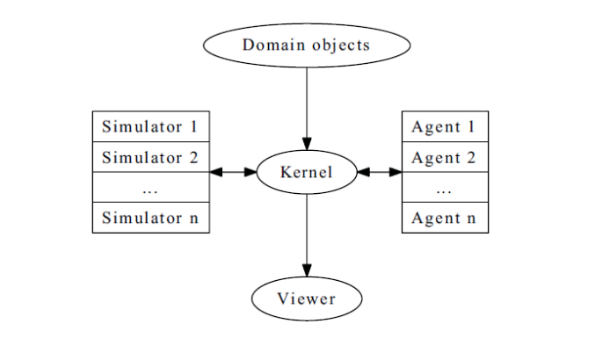
\includegraphics[scale=0.3]{fig1.png}}
\caption{RoboCup Rescue Agent Simulation platform architecture \cite{b1}}
\label{fig}
\end{figure}

A composição do server é entre 6 simuladores:
\begin{itemize}
\item \textit {Clear Simulator} - Responsável pela remoção de bloqueios das estradas. 
\item \textit {Collapse Simulator} - Responsável por gerenciar os danos estruturais dos prédios para criar bloqueios.
\item \textit {Ignition Simulator} - Realiza o princípio de incêndio nos prédios durante a simulação.
\item \textit {Fire Simulator} - Responsável por espalhar o fogo entre os edifícios.
\item \textit {Traffic Simulator} - Simulador responsável pelo movimento das entidades humanas.
\item \textit {Misc Simulator} - Responsável pelo dano de humanos e estruturas.
\end{itemize}

Na arquitetura do ambiente, como visto na Fig 1, ainda estão os objetos da cena, que estão dispostos em um arquivo ponto .gml, onde estão todas as estruturas e vias do mapa. O "Viewer" seria uma visualização gráfica do sistema, onde estão sendo atualizados os agentes e estruturas no ambiente. 

Já os agentes são responsáveis pelas ações que alteram o ambiente, onde enviam ações para o kernel, ele gerencia a comunicação com o determinado simulador responsável pela ação e atualiza o "Viewer" de acordo com a situação atual do ambiente, mais detalhes serão explicados na seção sobres os Agentes e o ambiente.
\subsection{Eclipse - Linguagem Java}
A própria ferramenta tem bibliotecas e samples são todas feitas em Java, portanto foi facilmente a linguagem escolhida para o trabalho. No Robocup Rescue a atuação das equipes que participam do evento é na formulação de estratégias entre os agentes e de agentes com o ambiente. Portanto o desafio é gerenciar todas essas variantes programaticamente. 
O código é composto de classes auxiliares e classes do código dos Agentes. A função do eclipse é compilar este código e carregar os agentes ao Simulation Server, onde após isso os algoritmos serão executados no kernel do simulador, por fim atuando na simulação.

\subsection{JOSM Editor}
\textit {JOSM Editor - Java OpenStreetMap Editor} é a ferramenta utilizada para criar o nosso ambiente,que é o mapa que contém prédios e vias.É uma ferramenta de software livre, onde é possivel selecionar uma área em qualquer lugar mapa-mundi e é feita a classificação dos objetos em uma área.

IMG DE UM MAPA SENDO EDITADO NO JOSM

No nosso projeto, utilizamos a ferramenta para criar um mapa da UNESP Júlio de Mesquita Filho, onde tivemos que retirar muitos detalhes do mapa, para que o Simulation Server utilize corretamente os objetos do mapa.Portando das diversas classificações encontradas no JOSM o simulador só utilizará os prédios e vias, as mesmas foram melhor adaptadas para a performace da simulação.

\section{Ambiente - Entidades do Ambiente}
O ambiente é o lugar onde os agentes e simuladores interagem, onde ocorre a simulação. E que no caso deste projeto é representado por um mapa, onde há edifícios e vias.
\subsection{Bloqueios}
Bloqueios são entidades que bloqueiam os caminhos nas vias, portanto dificultando a movimentação dos agentes.
Eles são gerados pelo \textit{Collapse Simulator} de acordo com o dano aos edifícios, simulando assim detritos e prédios entrando em colapso em uma situação de desastre.
\subsection{Área}

\subsection{Edifícios}

\subsection{Figures and Tables}
\paragraph{Positioning Figures and Tables} Place figures and tables at the top and 
bottom of columns. Avoid placing them in the middle of columns. Large 
figures and tables may span across both columns. Figure captions should be 
below the figures; table heads should appear above the tables. Insert 
figures and tables after they are cited in the text. Use the abbreviation 
``Fig.~\ref{fig}'', even at the beginning of a sentence.

\begin{table}[htbp]
\caption{Table Type Styles}
\begin{center}
\begin{tabular}{|c|c|c|c|}
\hline
\textbf{Table}&\multicolumn{3}{|c|}{\textbf{Table Column Head}} \\
\cline{2-4} 
\textbf{Head} & \textbf{\textit{Table column subhead}}& \textbf{\textit{Subhead}}& \textbf{\textit{Subhead}} \\
\hline
copy& More table copy$^{\mathrm{a}}$& &  \\
\hline
\multicolumn{4}{l}{$^{\mathrm{a}}$Sample of a Table footnote.}
\end{tabular}
\label{tab1}
\end{center}
\end{table}

\begin{figure}[htbp]
%\centerline{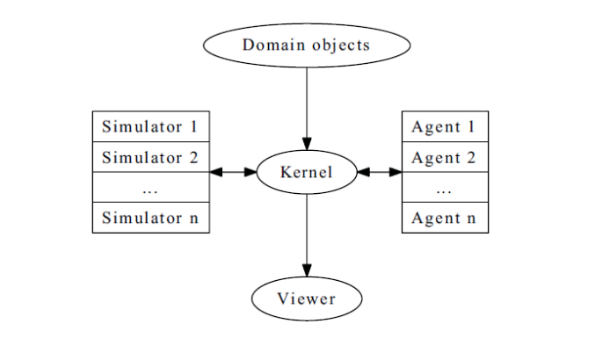
\includegraphics{fig1.png}}
\caption{Example of a figure caption.}
\label{fig}
\end{figure}

Figure Labels: Use 8 point Times New Roman for Figure labels. Use words 
rather than symbols or abbreviations when writing Figure axis labels to 
avoid confusing the reader. As an example, write the quantity 
``Magnetization'', or ``Magnetization, M'', not just ``M''. If including 
units in the label, present them within parentheses. Do not label axes only 
with units. In the example, write ``Magnetization (A/m)'' or ``Magnetization 
\{A[m(1)]\}'', not just ``A/m''. Do not label axes with a ratio of 
quantities and units. For example, write ``Temperature (K)'', not 
``Temperature/K''.

\section{Agentes}
Os agentes são os atores no nosso simulador, que interagem com o sistema e comunicam entre si. Nesta seção serão explicados as ações e funções de cada um.
\subsection{Civillians}
\subsection{Police Force}
\subsection{Fire Brigade}
\subsection{Ambulance Team}

\section{Comunicação? Estratégia?}

\section*{Acknowledgment}

The preferred spelling of the word ``acknowledgment'' in America is without 
an ``e'' after the ``g''. Avoid the stilted expression ``one of us (R. B. 
G.) thanks $\ldots$''. Instead, try ``R. B. G. thanks$\ldots$''. Put sponsor 
acknowledgments in the unnumbered footnote on the first page.

\section*{References}

Please number citations consecutively within brackets \cite{b1}. The 
sentence punctuation follows the bracket \cite{b2}. Refer simply to the reference 
number, as in \cite{b3}---do not use ``Ref. \cite{b3}'' or ``reference \cite{b3}'' except at 
the beginning of a sentence: ``Reference \cite{b3} was the first $\ldots$''

Number footnotes separately in superscripts. Place the actual footnote at 
the bottom of the column in which it was cited. Do not put footnotes in the 
abstract or reference list. Use letters for table footnotes.

Unless there are six authors or more give all authors' names; do not use 
``et al.''. Papers that have not been published, even if they have been 
submitted for publication, should be cited as ``unpublished'' \cite{b4}. Papers 
that have been accepted for publication should be cited as ``in press'' \cite{b5}. 
Capitalize only the first word in a paper title, except for proper nouns and 
element symbols.

For papers published in translation journals, please give the English 
citation first, followed by the original foreign-language citation \cite{b6}.

\begin{thebibliography}{00}
\bibitem{b1} G. Eason, B. Noble, and I. N. Sneddon, ``On certain integrals of Lipschitz-Hankel type involving products of Bessel functions,'' Phil. Trans. Roy. Soc. London, vol. A247, pp. 529--551, April 1955.
\bibitem{b2} J. Clerk Maxwell, A Treatise on Electricity and Magnetism, 3rd ed., vol. 2. Oxford: Clarendon, 1892, pp.68--73.
\bibitem{b3} I. S. Jacobs and C. P. Bean, ``Fine particles, thin films and exchange anisotropy,'' in Magnetism, vol. III, G. T. Rado and H. Suhl, Eds. New York: Academic, 1963, pp. 271--350.
\bibitem{b4} K. Elissa, ``Title of paper if known,'' unpublished.
\bibitem{b5} R. Nicole, ``Title of paper with only first word capitalized,'' J. Name Stand. Abbrev., in press.
\bibitem{b6} Y. Yorozu, M. Hirano, K. Oka, and Y. Tagawa, ``Electron spectroscopy studies on magneto-optical media and plastic substrate interface,'' IEEE Transl. J. Magn. Japan, vol. 2, pp. 740--741, August 1987 [Digests 9th Annual Conf. Magnetics Japan, p. 301, 1982].
\bibitem{b7} M. Young, The Technical Writer's Handbook. Mill Valley, CA: University Science, 1989.
\end{thebibliography}
\vspace{12pt}
\color{red}
IEEE conference templates contain guidance text for composing and formatting conference papers. Please ensure that all template text is removed from your conference paper prior to submission to the conference. Failure to remove the template text from your paper may result in your paper not being published.

\end{document}
